WebSocketはHTML5の重要な特徴です。これはブラウザに基づいたリモートsocketを実現します。ブラウザとサーバが全二重通信することができ、多くのブラウザ(Firefox、Google ChromeとSafari)ではすでにサポートされています。

WebSocketが現れる前はリアルタイム通信を実現するために、"ポーリング"とよばれる技術が全面的に採用されていました。すなわち、特定の時間間隔においてブラウザがサーバに対しHTTP Requestを送信し、サーバはリクエストを受け取った後、最新のデータをブラウザに返してリロードします。"ポーリング"ではブラウザがサーバに対して絶え間なくリクエストを送っており、大量の帯域幅を占有します。

WebSocketは特殊なパケットヘッダを採用しています。ブラウザとサーバはハンドシェイクの動作のみを必要とするだけで、ブラウザとサーバ間で接続チャンネルを確立することができます。またこの接続では活動状態が保持され、JavaScriptを使用することでコネクションに書き込むことも、中からデータを取り出すこともできます。通常のTCP Scoketを使用するのと同じようなものです。これはWebのリアルタイム化の問題を解決しています。伝統的なHTTPに比べ下のようなメリットがあります:

\begin{itemize}
  \item WebクライアントはTCP接続を確立するだけです
  \item Websocketサーバーはデータをwebクライアントにプッシュ(push)できます
  \item 軽いヘッダによりデータの転送量を抑えます。
\end{itemize}

WebSocket URLのはじめの入力はws://またはwss://(SSL上で)です。下の図はWebSocketの通信課程を示しています。特定のヘッダを伴ったHTTPハンドシェイクがサーバに送信され、サーバまたはクライアントはJavaScriptを使って何らかのソケット(socket)を使用します。このインターフェースはイベントを通して非同期にデータを受け取ることができます。

\begin{figure}[H]
  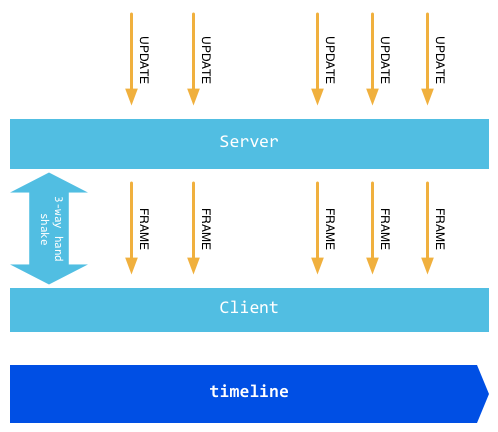
\includegraphics[width=14cm]{8.2.websocket.png}
  \label{図8.2}
   \caption{WebSocketの原理図}
\end{figure}



